\documentclass[fleqn]{article}

\usepackage{caption}
\usepackage{fancyhdr}
\usepackage{mathtools}
\usepackage{amsmath}
\usepackage{amssymb}
\usepackage{float}
\usepackage{tikz-timing}
\usepackage{longtable}
\usepackage{xepersian}

\settextfont[BoldFont={XB Zar bold.ttf}]{XB Zar.ttf}
\setlength\parindent{0pt}

\title{

\includegraphics[width=0.4\textwidth]{sharif.png}\\
\normalsize{دانشکده مهندسی کامپیوتر}\\
\vspace{1cm}
	
\huge{طراحی سیستم‌های دیجیتال}
\\
\Large{مستندات آزمون پایانترم}
\\
}

\author{
\\
استاد : دکتر اجلالی
\\
\\
پارسا محمدیان --- 98102284
}

\date{\today}

\begin{document}

\clearpage\maketitle
\thispagestyle{empty}

\newpage

\pagestyle{fancy}
\lhead{طراحی سیستم‌های دیجیتال}

\rhead{مستندات آزمون پایانترم}

\tableofcontents

\setcounter{page}{1}

\newpage

\section{سوال سه}
ابتدا مدار را ساده‌تر و بدون
\lr{CB} و \lr{SB}
رسم می‌کنیم. (شکل \ref{3simple})

\begin{figure}[!htbp]
	\centering
	
\includegraphics[width=\linewidth]{3simple.png}
	\caption{ساده شده مدار \lr{FPGA}}
	\label{3simple}
\end{figure}

همانطور که از شکل 
\ref{3simple}
مشخص است مدار ترتیبی است، چون خروجی به غیر از ورودی به حالت‌ها (مقدار فلیپ فلاپ‌ها) نیز وابسته است. 

حال به کمک جدول \lr{LUT} جدول حالت را بدست می‌آوریم.

در این جدول 
\lr{$Q_{11}$}
مقدار فعلی فلیپ فلاپ کنار 
\lr{LUT 11}
،
\lr{$Q_{12}$}
مقدار فعلی فلیپ فلاپ کنار 
\lr{LUT 12}
و
\lr{$Q_{22}$}
مقدار فعلی فلیپ فلاپ کنار 
\lr{LUT 22}
هستند و 
\lr{$Q_{11}^+$}
مقدار بعدی فلیپ فلاپ کنار 
\lr{LUT 11}
،
\lr{$Q_{12}^+$}
مقدار بعدی فلیپ فلاپ کنار 
\lr{LUT 12}
و
\lr{$Q_{22}^+$}
مقدار بعدی فلیپ فلاپ کنار 
\lr{LUT 22}
هستند.

\begin{latin}
	\begin{center}
		\begin{longtable}{|ccc|ccc||ccc|c|}
			\hline
			$Q_{11}$ & $Q_{12}$ & $Q_{22}$ & A & B & C & $Q_{11}^+$ & $Q_{12}^+$ & $Q_{22}^+$ & out \\ \hline \hline
			0        & 0        & 0        & 0 & 0 & 0 & 0          & 0          & 1          & 0   \\ \hline
			0        & 0        & 0        & 0 & 0 & 1 & 0          & 1          & 0          & 0   \\ \hline
			0        & 0        & 0        & 0 & 1 & 0 & 1          & 0          & 0          & 0   \\ \hline
			0        & 0        & 0        & 0 & 1 & 1 & 1          & 1          & 1          & 0   \\ \hline
			0        & 0        & 0        & 1 & 0 & 0 & 1          & 0          & 0          & 0   \\ \hline
			0        & 0        & 0        & 1 & 0 & 1 & 1          & 1          & 1          & 0   \\ \hline
			0        & 0        & 0        & 1 & 1 & 0 & 0          & 0          & 1          & 0   \\ \hline
			0        & 0        & 0        & 1 & 1 & 1 & 0          & 1          & 0          & 0   \\ \hline
			0        & 0        & 1        & 0 & 0 & 0 & 0          & 0          & 1          & 1   \\ \hline
			0        & 0        & 1        & 0 & 0 & 1 & 0          & 1          & 0          & 1   \\ \hline
			0        & 0        & 1        & 0 & 1 & 0 & 1          & 0          & 0          & 1   \\ \hline
			0        & 0        & 1        & 0 & 1 & 1 & 1          & 1          & 1          & 1   \\ \hline
			0        & 0        & 1        & 1 & 0 & 0 & 1          & 0          & 0          & 1   \\ \hline
			0        & 0        & 1        & 1 & 0 & 1 & 1          & 1          & 1          & 1   \\ \hline
			0        & 0        & 1        & 1 & 1 & 0 & 0          & 0          & 1          & 1   \\ \hline
			0        & 0        & 1        & 1 & 1 & 1 & 0          & 1          & 0          & 1   \\ \hline
			0        & 1        & 0        & 0 & 0 & 0 & 0          & 0          & 0          & 0   \\ \hline
			0        & 1        & 0        & 0 & 0 & 1 & 0          & 1          & 1          & 0   \\ \hline
			0        & 1        & 0        & 0 & 1 & 0 & 1          & 0          & 1          & 0   \\ \hline
			0        & 1        & 0        & 0 & 1 & 1 & 1          & 1          & 0          & 0   \\ \hline
			0        & 1        & 0        & 1 & 0 & 0 & 1          & 0          & 1          & 0   \\ \hline
			0        & 1        & 0        & 1 & 0 & 1 & 1          & 1          & 0          & 0   \\ \hline
			0        & 1        & 0        & 1 & 1 & 0 & 0          & 0          & 0          & 0   \\ \hline
			0        & 1        & 0        & 1 & 1 & 1 & 0          & 1          & 1          & 0   \\ \hline
			0        & 1        & 1        & 0 & 0 & 0 & 0          & 0          & 0          & 1   \\ \hline
			0        & 1        & 1        & 0 & 0 & 1 & 0          & 1          & 1          & 1   \\ \hline
			0        & 1        & 1        & 0 & 1 & 0 & 1          & 0          & 1          & 1   \\ \hline
			0        & 1        & 1        & 0 & 1 & 1 & 1          & 1          & 0          & 1   \\ \hline
			0        & 1        & 1        & 1 & 0 & 0 & 1          & 0          & 1          & 1   \\ \hline
			0        & 1        & 1        & 1 & 0 & 1 & 1          & 1          & 0          & 1   \\ \hline
			0        & 1        & 1        & 1 & 1 & 0 & 0          & 0          & 0          & 1   \\ \hline
			0        & 1        & 1        & 1 & 1 & 1 & 0          & 1          & 1          & 1   \\ \hline
			1        & 0        & 0        & 0 & 0 & 0 & 0          & 1          & 0          & 0   \\ \hline
			1        & 0        & 0        & 0 & 0 & 1 & 0          & 0          & 1          & 0   \\ \hline
			1        & 0        & 0        & 0 & 1 & 0 & 1          & 1          & 1          & 0   \\ \hline
			1        & 0        & 0        & 0 & 1 & 1 & 1          & 0          & 0          & 0   \\ \hline
			1        & 0        & 0        & 1 & 0 & 0 & 1          & 1          & 1          & 0   \\ \hline
			1        & 0        & 0        & 1 & 0 & 1 & 1          & 0          & 0          & 0   \\ \hline
			1        & 0        & 0        & 1 & 1 & 0 & 0          & 1          & 0          & 0   \\ \hline
			1        & 0        & 0        & 1 & 1 & 1 & 0          & 0          & 1          & 0   \\ \hline
			1        & 0        & 1        & 0 & 0 & 0 & 0          & 1          & 0          & 1   \\ \hline
			1        & 0        & 1        & 0 & 0 & 1 & 0          & 0          & 1          & 1   \\ \hline
			1        & 0        & 1        & 0 & 1 & 0 & 1          & 1          & 1          & 1   \\ \hline
			1        & 0        & 1        & 0 & 1 & 1 & 1          & 0          & 0          & 1   \\ \hline
			1        & 0        & 1        & 1 & 0 & 0 & 1          & 1          & 1          & 1   \\ \hline
			1        & 0        & 1        & 1 & 0 & 1 & 1          & 0          & 0          & 1   \\ \hline
			1        & 0        & 1        & 1 & 1 & 0 & 0          & 1          & 0          & 1   \\ \hline
			1        & 0        & 1        & 1 & 1 & 1 & 0          & 0          & 1          & 1   \\ \hline
			1        & 1        & 0        & 0 & 0 & 0 & 0          & 1          & 1          & 0   \\ \hline
			1        & 1        & 0        & 0 & 0 & 1 & 0          & 0          & 1          & 0   \\ \hline
			1        & 1        & 0        & 0 & 1 & 0 & 1          & 1          & 0          & 0   \\ \hline
			1        & 1        & 0        & 0 & 1 & 1 & 1          & 0          & 1          & 0   \\ \hline
			1        & 1        & 0        & 1 & 0 & 0 & 1          & 1          & 0          & 0   \\ \hline
			1        & 1        & 0        & 1 & 0 & 1 & 1          & 0          & 1          & 0   \\ \hline
			1        & 1        & 0        & 1 & 1 & 0 & 0          & 1          & 1          & 0   \\ \hline
			1        & 1        & 0        & 1 & 1 & 1 & 0          & 0          & 0          & 0   \\ \hline
			1        & 1        & 1        & 0 & 0 & 0 & 0          & 1          & 1          & 1   \\ \hline
			1        & 1        & 1        & 0 & 0 & 1 & 0          & 0          & 1          & 1   \\ \hline
			1        & 1        & 1        & 0 & 1 & 0 & 1          & 1          & 0          & 1   \\ \hline
			1        & 1        & 1        & 0 & 1 & 1 & 1          & 0          & 1          & 1   \\ \hline
			1        & 1        & 1        & 1 & 0 & 0 & 1          & 1          & 0          & 1   \\ \hline
			1        & 1        & 1        & 1 & 0 & 1 & 1          & 0          & 1          & 1   \\ \hline
			1        & 1        & 1        & 1 & 1 & 0 & 0          & 1          & 1          & 1   \\ \hline
			1        & 1        & 1        & 1 & 1 & 1 & 0          & 0          & 0          & 1   \\ \hline
		\end{longtable}
	\end{center}
\end{latin}

حال با توجه به جدول حالت نمودار حالت را رسم می‌کنیم. (شکل \ref{stateDiagram3})
در شکل 
\ref{stateDiagram3}
حالت‌ها با کدهای باینری که از کنار هم گذاشتن خروجی فلیپ فلاپ بدست می‌آید شماره‌گذاری شده‌اند.

$$
\text{شماره حالت} = \overline{Q_{11} Q_{12} Q_{22}}
$$

\begin{figure}[!htbp]
	\centering
	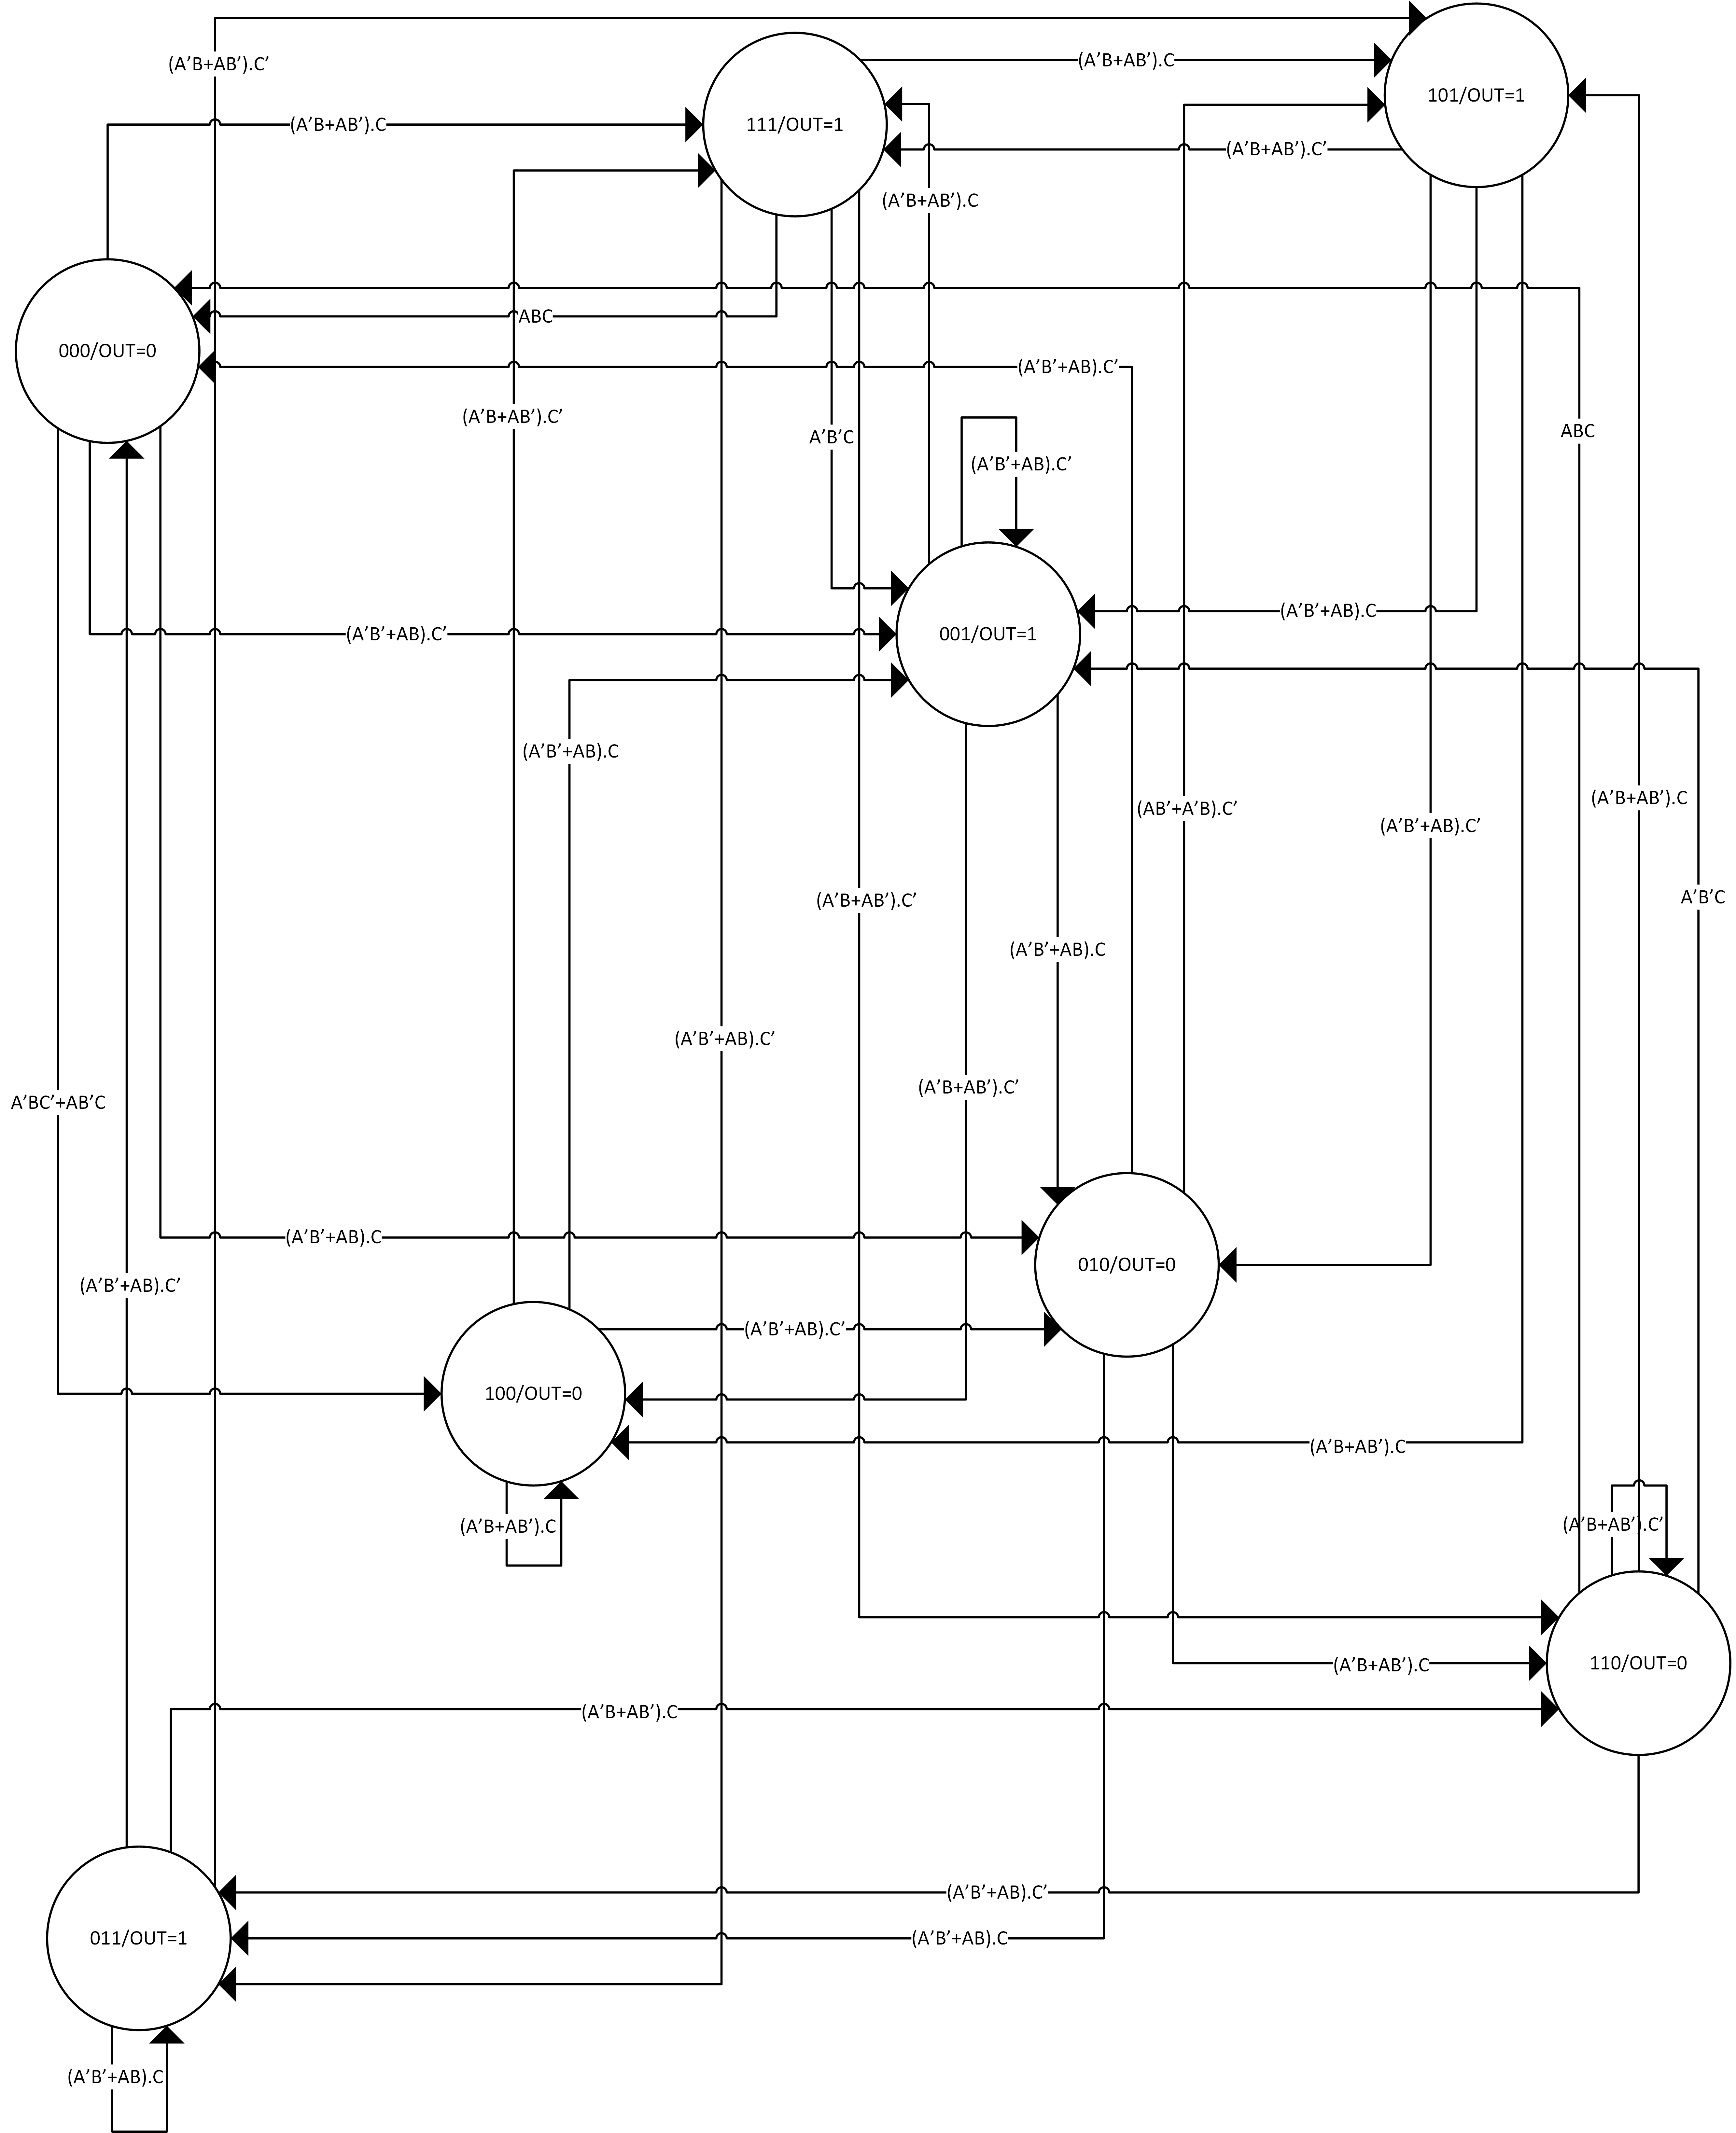
\includegraphics[width=\linewidth]{3stateDiagram.png}
	\caption{نمودار حالت کشیده شده از روی جدول حالت}
	\label{stateDiagram3}
\end{figure}

از آنجایی که 3 ورودی داریم به صورت کلی از هر حالت سه یال به حالات دیگر خارج می‌شود. حال 
با ساده‌سازی (ادغام یال‌هایی که مبدا و مقصد مشترک دارند و شروطشان) این یال‌ها کمتر می‌شوند.

\section{سوال شش}
\subsection{شرط ورودی \lr{In} نسبت به \lr{CLK}}
در حالت کلی، هر تغییر ورودی
\lr{In}
باید تا
\lr{triger}
شدن کلاک باقی بماند تا اثرش دیده شود.

اگر فرض کنیم ورودی
\lr{In}
تغییر می‌کند، و قبل از
\lr{triger}
شدن کلاک، زوج بار تغییر می‌کند، آنگاه وقتی با
\lr{triger}
شدن کلاک با مقدار قبلی خود (به منظور کشف تغییر) مقایسه می‌شود، چون زوج بار تغییر کرده است نتیجه مقایسه برابری
است. پس در این صورت اصلا تغییرات شمرده نمی‌شوند.

از طرفی دیگر اگر فرض کنیم ورودی
\lr{In}
تغییر می‌کند، و قبل از
\lr{triger}
شدن کلاک، فرد بار تغییر می‌کند، آنگاه وقتی با
\lr{triger}
شدن کلاک با مقدار قبلی خود (به منظور کشف تغییر) مقایسه می‌شود، نتیجه مقایسه نشان می‌دهد نسبت به مقدار قبلی خود
تغییر کرده است و یک تغییر شمرده می‌شود. در حالیکه می‌دانیم ممکن است بیش از یک بار (مثلا 5 بار) تغییر کرده باشد.

\subsection{توصیف رفتاری}
جزئیات پیاده‌سازی در فایل
\lr{transmition\_counter.v}
موجود است. در این ماژول قسمتی که از سیستم تسک برای چاپ خطا بر روی صفحه استفاده شده قابل سنتز نبوده و
تنها در شبیه‌سازی عمل می‌کند. توجه شود که چک کردن خطا در لبه بالارونده کلاک انجام می‌شود.

\subsection{شبیه‌سازی و تست کد}
برای اطمینان از صحت عملکرد مدار، تست بنچ در فایل
\lr{transmition\_counter\_tb.v}
نوشته شده است. در قسمت اول آن تغییرات از شرط بخش الف پیروی می‌کنند پس تغییرات به درستی شمرده می‌شوند و
خطایی رخ نمی‌دهد. در قسمت دوم که تغییرات مطابق شرط بخش اول نیستند خطای مناسب چاپ می‌شود.

جزئیات اجرای شبیه‌سازی در شکل
\ref{simulate6}
قابل مشاهده است.

\begin{figure}[!htbp]
	\centering
	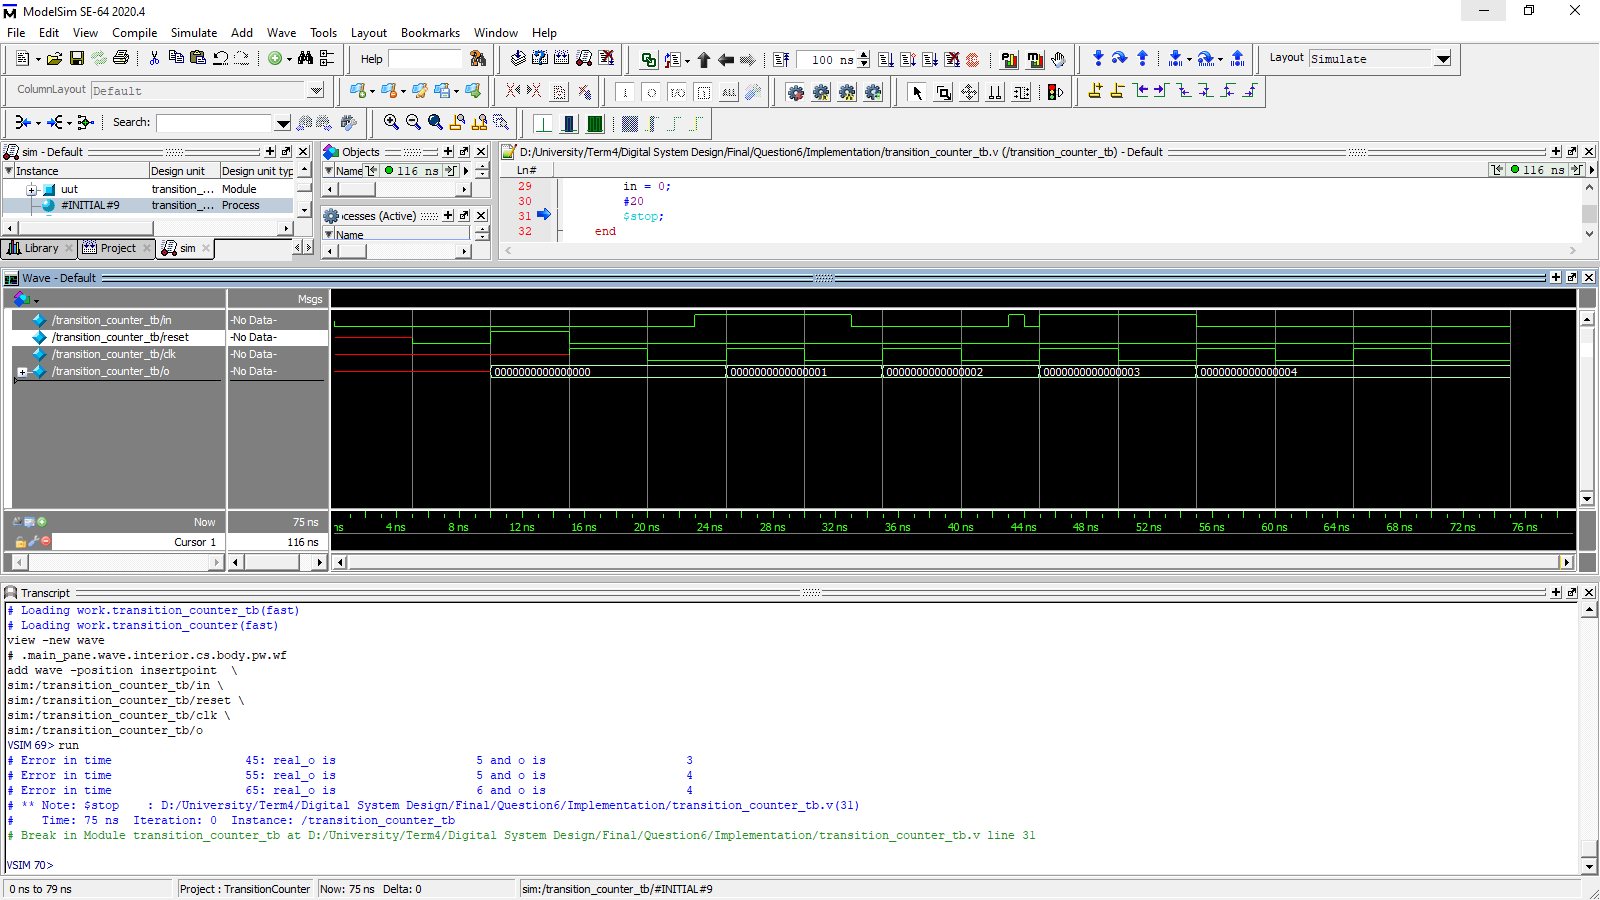
\includegraphics[width=\linewidth]{6.png}
	\caption{نتیجه اجرای شبیه‌سازی \lr{transition counter}}
	\label{simulate6}
\end{figure}

\section{سوال هفت}
\subsection{پیاده‌سازی برنامه پایتون}
برنامه نوشته شده که در فایل
\lr{dataflow2behavioral/main.py}
موجود است به صورت
\begin{latin}
	python main.py -i <inputFile> -o <outputFile>
\end{latin}
اجرا شده و
\lr{inputFile}
را مورد پردازش قرار می‌دهد و حاصل را در
\lr{outputFile}
می‌ریزد. بیشتر پردازش‌ها توسط
\lr{Regex}
انجام شده است.

\subsection{تست کردن برنامه}

\subsubsection{تست فرضی}
در این تست یک برنامه فرضی نوشته شده که از انواع
\lr{Continues Assignment}
ها استفاده می‌کند. این کد را با برنامه پایتون به کد رفتاری تبدیل می‌کنیم. سپس ماژولی برای تست آن به این صورت
می‌نویسیم که تمام حالات ورودی را مقداردهی کند سپس خروجی دو ماژول رفتاری و جریان داده را از طریق
شکل موج مقایسه می‌کنیم. کدهای جریان داده، رفتاری و تست به ترتیب در فایل‌های
\lr{dataflow.v}
و
\lr{behavioral.v}
و
\lr{testbench.v}
موجود هستند. نتیجه اجرای
\lr{testbench}
نیز در شکل
\ref{test1for7}
قابل مشاهده است.

\begin{figure}[!htbp]
	\centering
	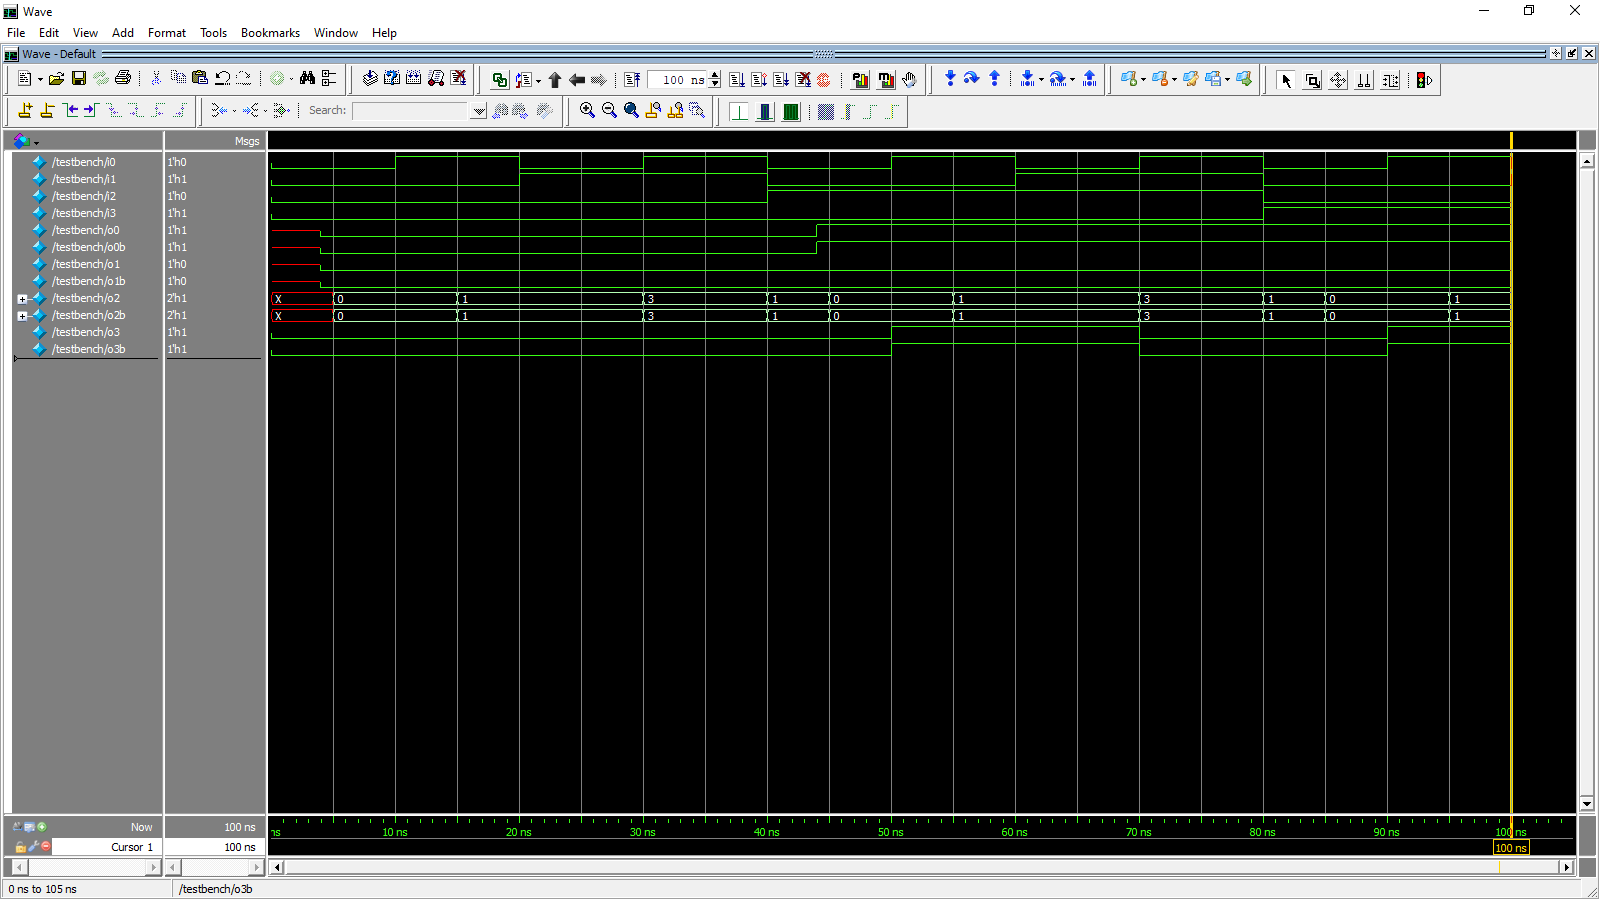
\includegraphics[width=\linewidth]{7test1.png}
	\caption{همانطور که مشاهده می‌شود خروجی‌های متناظر کاملا یکسان هستند. (دقت شود که خروجی‌های \lr{oi} مربوط به توصیف جریان داده و خروجی‌های \lr{oib} مربوط به توصیف رفتاری هستند)}
	\label{test1for7}
\end{figure}

\subsubsection{تست عملیاتی}
حال کد تمرین 5 هیمن درس که یک واحد
\lr{dff}
به صورت جریان داده بود را مورد تست قرار می‌دهیم. باز هم مشاهده می‌شود که شکل موج خروجی‌ها کاملا یکسان است. (شکل \ref{test2for7})

\begin{figure}[!htbp]
	\centering
	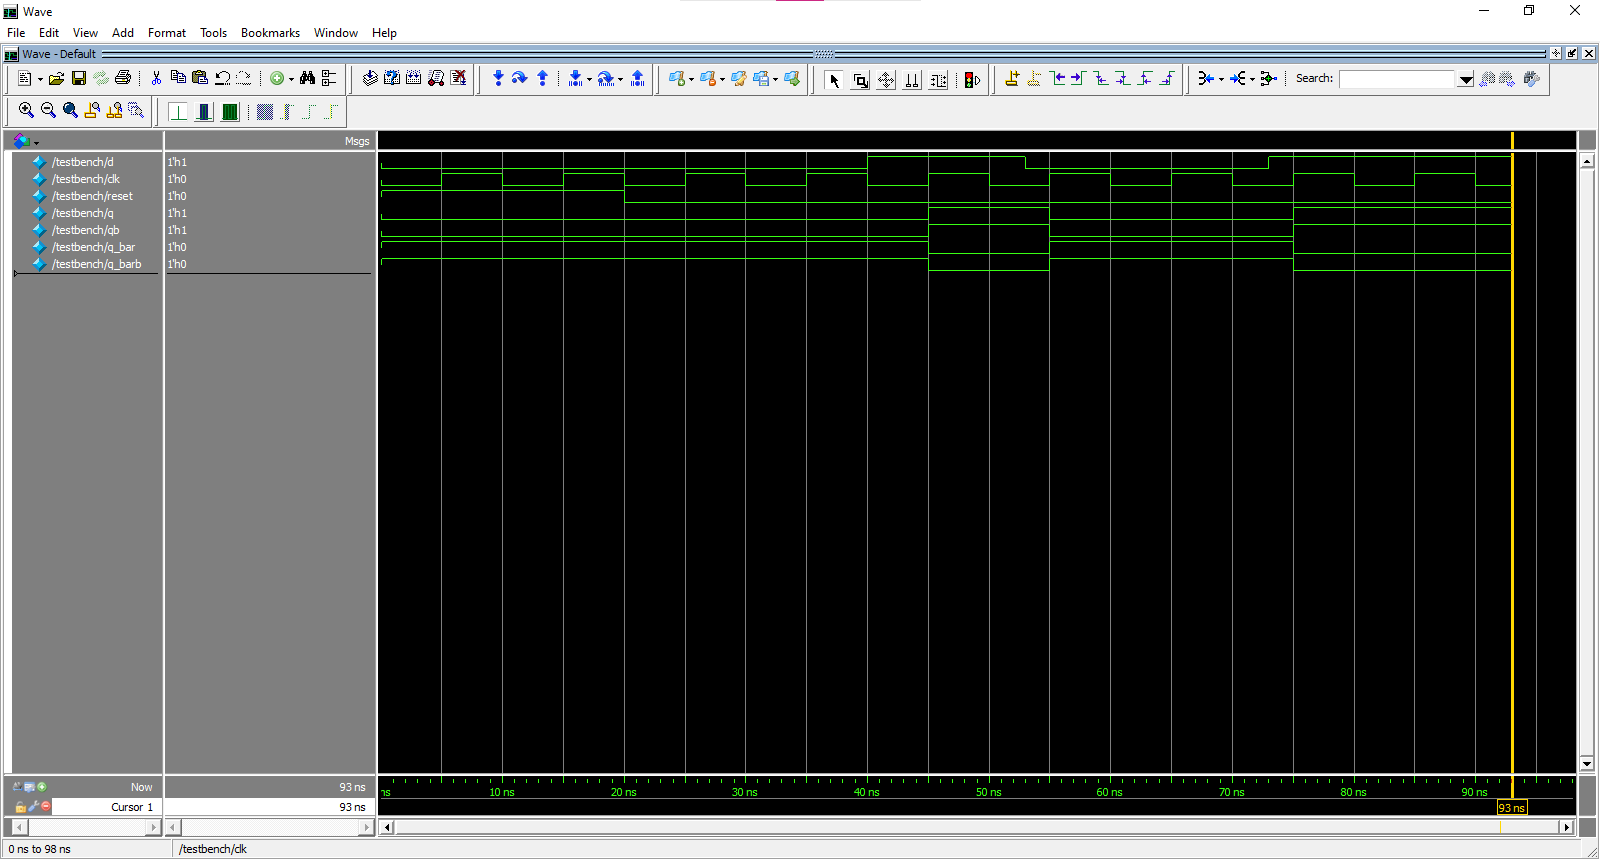
\includegraphics[width=\linewidth]{7test2.png}
	\caption{همانطور که مشاهده می‌شود خروجی‌های متناظر کاملا یکسان هستند. (دقت شود که خروجی‌های \lr{x} مربوط به توصیف جریان داده و خروجی‌های \lr{xb} مربوط به توصیف رفتاری هستند)}
	\label{test2for7}
\end{figure}

\end{document}